\documentclass[12pt]{article}

\usepackage[utf8]{inputenc}
\usepackage[T1]{fontenc}

\usepackage{geometry}
\geometry{
    a4paper,
    total={150mm, 247mm},
    left={30mm},
    top={25mm}
}
\usepackage[english,czech]{babel}
\usepackage{mathpazo}
\usepackage{graphicx}
\usepackage{hyperref}
\usepackage{wrapfig}
\usepackage[
backend=bibtex,
style=iso-numeric,
currentlang=true,
sorting=ynt
]{biblatex} %Imports biblatex package
\addbibresource{citations.bib} %Import the bibliography file
\usepackage[automake, acronym, toc]{glossaries}
\graphicspath{ {./attachments} }

\makeatletter
\renewcommand{\fnum@figure}{Obr.: \thefigure}
\makeatother

\makeglossaries

\renewcommand{\contentsname}{Obsah}
\renewcommand{\listfigurename}{Seznam obrázků}
\renewcommand{\listtablename}{Seznam tabulek}
\renewcommand{\refname}{Zdroje}

\title{OpenOscilloscopeModule}
\author{Daniel Židek}
\date{Září 2023}

\begin{document}

%\newacronym{label}{acronym}{whole phrase}
%           [longplural={whole phrases},shortplural=labels]

%\acrshort{lcd}      - LCD
%\acrlong{lcd}       - Liquid Crystal Display
%\acrfull{lcd}       - Liquid Crystal Display (LCD)

%\acrshortpl{lcd}    - LCDs
%\acrlongpl{lcd}     - Liquid Crystal Displays
%\acrfullpl{lcd}     - Liquid Crystal Displays (LCDs)


\newacronym{lcd}{LCD}{Liquid Crystal Display}
\newacronym[longplural={Časové Základny},shortplural=ČZ]{casz}{ČZ}{Časová Základna}
\newglossaryentry{trigger}
{
    name=trigger,
    description={Spouštěč, systém odpovědný za spuštění \acrlongpl{casz}}
}

% SPDX-FileCopyrightText: 2023 2023 Daniel Židek <danielzidek@post.cz>
%
% SPDX-License-Identifier: GPL-3.0-or-later

\begin{titlepage} % Suppresses displaying the page number on the title page and the subsequent page counts as page 1
	\newcommand{\HRule}{\rule{\linewidth}{0.5mm}} % Defines a new command for horizontal lines, change thickness here
	
	\center % Centre everything on the page
	
	%------------------------------------------------
	%	Headings
	%------------------------------------------------
	
	\textsc{\LARGE Daniel Židek}\\[1.5cm] % Main heading such as the name of your university/college
	
	\textsc{\Large OSModIn - Modulární laboratorní přístroje}\\[0.5cm] % Major heading such as course name
	
	\textsc{\large Technická dokumentace}\\[0.5cm] % Minor heading such as course title
	
	%------------------------------------------------
	%	Title
	%------------------------------------------------
	
	\HRule\\[0.4cm]
	
	{\huge\bfseries Zařízení modulární instrumentace}\\[0.4cm] % Title of your document
	
	\HRule\\[1.5cm]
	
	%------------------------------------------------
	%	Author(s)
	%------------------------------------------------
	
	\begin{minipage}{0.4\textwidth}
		\begin{flushleft}
			\large
			\textit{Autor}\\
			Daniel \textsc{Židek} % Your name
		\end{flushleft}
	\end{minipage}
	~
	\begin{minipage}{0.4\textwidth}
		\begin{flushright}
			\large
			\textit{Vedoucí práce}\\
			Daniel \textsc{Židek} % Supervisor's name
		\end{flushright}
	\end{minipage}
	
	% If you don't want a supervisor, uncomment the two lines below and comment the code above
	%{\large\textit{Author}}\\
	%John \textsc{Smith} % Your name
	
	%------------------------------------------------
	%	Date
	%------------------------------------------------
	
	\vfill\vfill\vfill % Position the date 3/4 down the remaining page
	
	{\large Září 2023} % Date, change the \today to a set date if you want to be precise
	
	%------------------------------------------------
	%	Logo
	%------------------------------------------------
	
	%\vfill\vfill
	%\includegraphics[width=0.2\textwidth]{placeholder.jpg}\\[1cm] % Include a department/university logo - this will require the graphicx package
	 
	%----------------------------------------------------------------------------------------
	
	\vfill % Push the date up 1/4 of the remaining page
	
\end{titlepage}

\setcounter{page}{2}

\tableofcontents

\newpage

\addcontentsline{toc}{section}{Seznam obrázků}
\renewcommand{\listfigurename}{Seznam obrázků}
\listoffigures

\newpage

\addcontentsline{toc}{section}{Seznam tabulek}
\renewcommand{\listtablename}{Seznam tabulek}
\listoftables

\newpage

\section{Abstrakt}

Tato práce se zabývá návrhem a realizací osciloskopu pod otevřenou licencí CERN-OHL-S v2.
Výsledkem by měl být osciloskop v Eurocard formátu, s šířkou pásma alespoň 60MHz, 
2 kanály a cenou do 12 tisíc CZK. Tato práce dokumentuje proces vývoje,
rozhodnutí a další poznámky týkající se ModIns Osciloskopu. Kromě toho zde
dokumentuji i proces seznamování se se zpracováním rychlých analogových
signálů a práce s FPGA - celý projekt vzniká jako záminka naučit se něco nového.
Celý projekt je hostovaný na GitHubu v repozitáři
\href{https://github.com/zidekd/OpenOscilloscopeModule}{zidekd/OpenOscilloscopeModule}.

\newpage

\section{Úvod}

Celý projekt začínám pro to, abych si zkusil něco nového.
Selhal a zkusil to znovu. Ve výsledku bych rád disponoval šasím
podobným PXI od National Instruments a několika moduly pro něj.
Jmenovitě je zatím plánovaný osciloskop a laboratorní zdroj.
Všechny přístroje budou disponovat univerzálním protokolem pro
komunikaci (kód tak bude moct být znovupoužitelný), komunikačními
linkami a především obslužným software pro MS Windows (XP a 10),
GNU+Linux a MacOS. Řídící jednotka bude moct sloužit také jako server,
který by dovoloval obsluhu přístrojů nejen lokálně, přes USB, WiFi či LAN
ale i sdílet přístroje reverzním tunelem. Zde bude otázka zabezpečení,
nicméně takový software by měl dovolovat přístup více uživatelů s
různými oprávněními (číst data z přístrojů, měnit jejich nastavení, ...).
To by mohlo být příhodné ve výuce, či na pracovištích s možností vzdálené práce.

Formát Eurocard jsem vybral pro to, protože mi přijde nejvhodnější.
Je tedy ještě potřeba domyslet použití konektorů a komunikačních protokolů,
ale o tom potom. :) Eurocard standard dovoluje použití modulů, jež jsou
ukládány do šasí které lze následně připevnit do 19 palcového racku. Velikost
racku jsou obvykle násobky tří, tedy 3U, 6U, atd.

Co se obslužného software týče tak by moduly měly podporovat ovládání
skrz Python API, vizuální grafické rozhraní připomínající ovládáním běžných
laboratorních přístrojů a také by měly moct být ovládány skrze vizuální editor 
zlú (podobný Node-RED, LabVIEW...). Ovládání skrze Python API, GUI i Node-based editor
bude možné jak lokálně přes USB, WiFi a LAN tak i přes reverzní tunel, kdy potom
lze ovládat přístroje i na druhém konci světa. Ačkoliv jde o sdílení "pouze" připojených
přístrojů, všechny aplikace schopné s takovým spojením interagovat budou podporovat
správu oprávnění a logů. Řídící jednotka bude zaznamenávat všechny akce, dle úrovní,
takže v závislosti na nastavení se budou ukládat různě závažné záznamy. Co do správy
oprávnění tak k dispozici bude několik úrovní přístupů a ty půjde omezit jak na
jednotlivé přístroje, tak na celé sestavy.

\newpage

\section{Teoretický úvod}

V následující kapitole rozeberu funkci analogových a digitálních osciloskopů, pokusím
se provést rozbor komerčních osciloskopů (alespoň dle reverzních schémat; u 
otevřených designů je tohle však mnohem jednodušší :D) a také porovnám
návrhy jednotlivých bloků, na základě čehož budu stavit vlastní návrh.

\subsection{Analogové osciloskopy}

Základní princip funkce spočívá ve vychylování elektronového paprsku měřeným
signálem a signálem \acrfullpl{casz}. Vychýlený elektronový paprsek následně
dopadá na speciální stínítko, které se v místě dopadu rozsvěcí. Analogové
osciloskopy se již nepoužívají, ačkoliv pozor, ne každý osciloskop s CRT obrazovkou
je analogový osciloskop. Pokud dnes osciloskop s CRT obrazovkou potkáte,
s největší pravděpodobnopstí jde o analogový paměťový osciloskop, nebo zkrátka
o \acrfull{dso}. Rozdíly mezi nimi rozeberu později.

\begin{figure}[h]
\centering
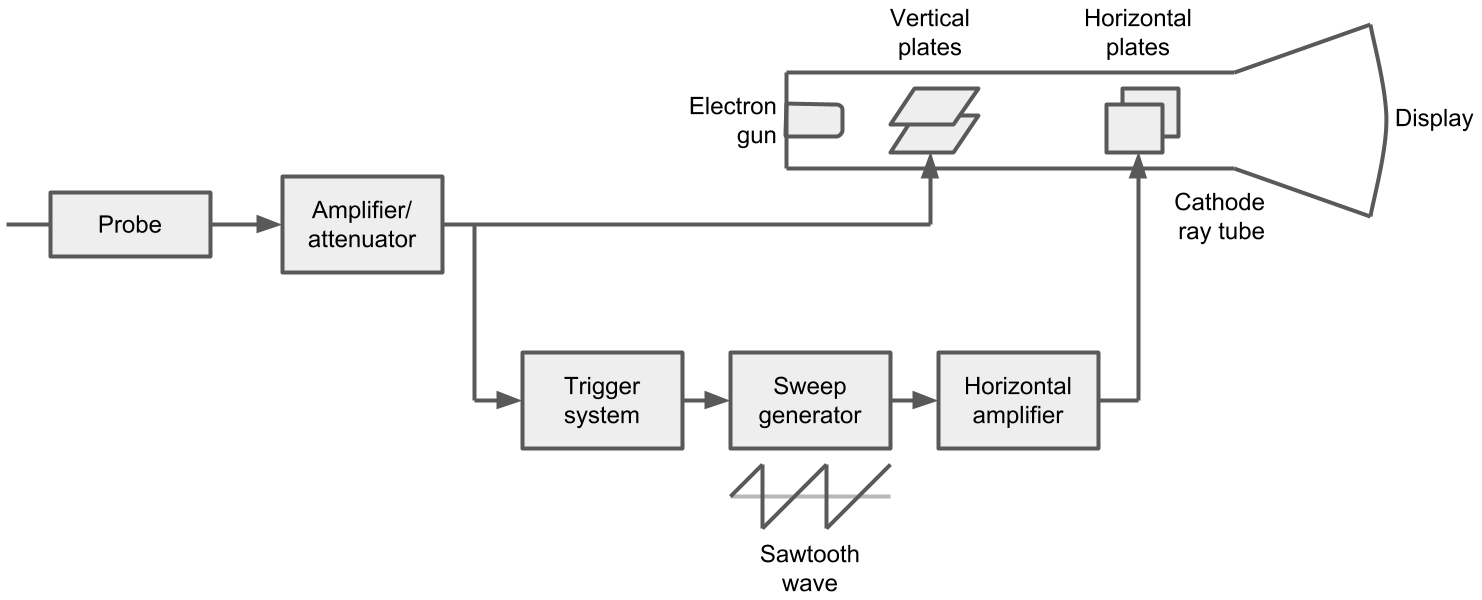
\includegraphics[width=\textwidth]{analog-oscilloscope-diagram}
\caption{Blokový diagram analogového osciloskopu (převzato z \cite{HowDoesOscilloscope})}
\label{fig:blok-analog-osci}
\end{figure}

\begin{wrapfigure}{r}{0.5\textwidth}
\centering
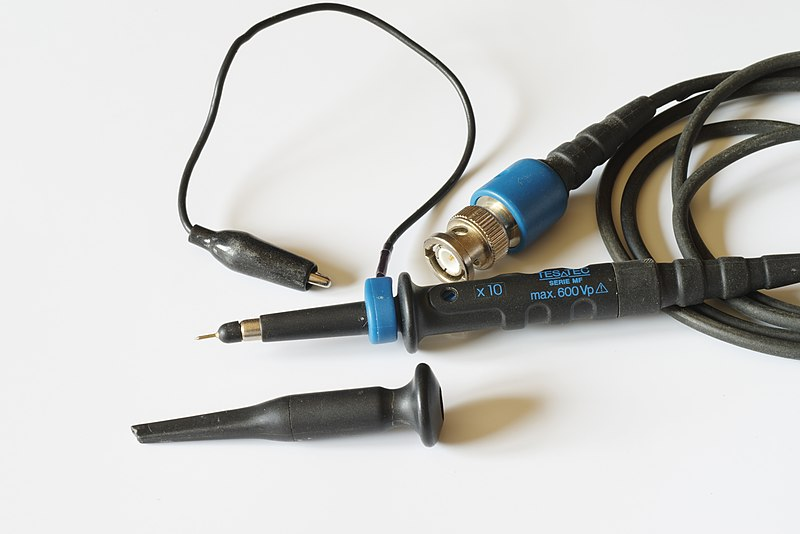
\includegraphics[width=0.5\textwidth]{osci-pasive-probe}
\caption{Pasivní sonda (převzato z \cite{DeutschStandardTastkopfFur2020})}
\label{fig:osci-pasive-probe}
\end{wrapfigure}

Na obrázku \ref{fig:blok-analog-osci} jako první vidíme blok "probe", tedy osciloskopickou
sondu. Ta slouží k samotnému měření. Obvykle říkáme pouze "sonda", z kontextu je
totiž jasné, o co jde. Nejčastěji se setkáme s pasivními sondami,
(na obr. \ref{fig:osci-pasive-probe}) to jsou sondy ideální na takové běžné měření
do 500 MHz a pravděpodobně to jsou i sondy, co přišly s vašim osciloskopem.
Dále máme atenuátory, což je část obvodu odpovědná za snížení amplitudy vstupního signálu.
Je-li vstupní signál příliš velký, můžeme využít právě atenuátoru pro snížení
amplitudy bez změny frekvence, či jiného zásahu do samotného tvaru signálu.
Atenuátor se obvykle vyskytuje jen po pár krocích, obvykle 1:4, 1:10 a 1:20.
V tomto blokovém schématu je spolu s atenuátorem spojen ještě zesilovač vertikální osy.
Ten se zase stará o spojitou regulaci signálu, abychom například využili celou výšku
zobrazovadla a to i signálem s nízkou amplitudou. Ze zesilovače signál
jde dále do \gls{trigger}u. Jeden z nejčastějčích obvodů pro spouštěcí systém je Schmittův
klopný obvod. Ten slouží ke spuštění tzv. sweep generátoru, tedy generátoru \acrfullpl{casz}.
Stejně jako u vstupního signálu i signál \acrshort{casz} pokračuje do zesilovače a z něj na
vychylovací destičky pro horizontální osu.

\subsubsection{Schmittův klopný obvod} \label{sec:schmitt-ko}

%TODO: Přesunout do samostatné sekce triggerů, spolu s dalšími obvody

Schmittův klopný obvod je speciální komparátor, který má hysterezi. To znamená, že jeho
výstup je závislý nejen na hodnotě vstupu, ale i na jeho původním stavu. Podobně jako
obyčejný komparátor s operačním zesilovačem, i Schmittův klopný obvod dosahuje na výstupu
kladného nebo záporného saturačního napětí.

Pokud je na výstupu například kladné napětí, nedojde k překlopení Schmittova obvodu
při pouhém splnění podmínky U+ < U- jako u komparátoru, ale teprve až rozdíl obou napětí
dosáhne prahové hodnoty H- . Podobně, pokud je nyní na výstupu záporné saturační napětí,
může dojít ke zpětnému překlopení Schmittova obvodu teprve až v momentě, kdy je U+ > U- o
více než H+. (Celá část \ref{sec:schmitt-ko} je převzata z \cite{ELUCNapetovyKomparator})

\begin{figure}[h]
    \centering
    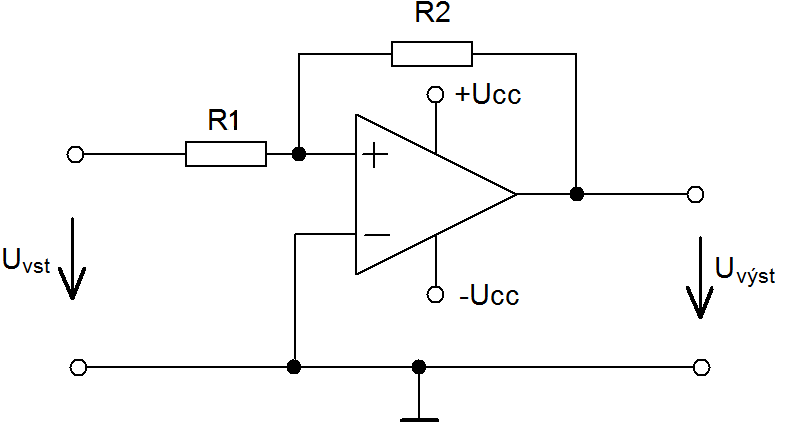
\includegraphics[width=0.5\textwidth]{schmitt-ko}
    \caption{Schmittův \acrshort{ko} pomocí \acrshort{nk}}
    \label{fig:schmitt-ko}
\end{figure}

\newpage

\printbibliography[
heading=bibintoc,
title={Seznam použité literatury}
]

\newpage

\printglossary[type=\acronymtype, title=Abecední seznam zkratek, toctitle=Abecední seznam zkratek]

\printglossary[title=Slovník pojmů, toctitle=Slovník pojmů]

\end{document}
